\documentclass[12pt,a4paper]{article}

%% ---- Packages ----
\usepackage{amsmath}
\usepackage{amssymb}
\usepackage{geometry}
\geometry{margin=2.5cm}
\usepackage{booktabs}
\usepackage{xcolor}
\usepackage{hyperref}
\usepackage{listings}
\usepackage{pgfplots}
\pgfplotsset{compat=1.18}
\usepackage[most,breakable]{tcolorbox}
\tcbuselibrary{skins, breakable}
\usepackage{enumitem}
\usepackage{fancyhdr}
\usepackage{tikz}
\usepackage{array}

%% ---- tcolorbox environments ----
\newtcolorbox{curiositybox}[1]{colback=yellow!10, colframe=orange!80!black, fonttitle=\bfseries, title=#1, breakable}
\newtcolorbox{infobox}[1]{colback=blue!5, colframe=blue!60!black, fonttitle=\bfseries, title=#1, breakable}
\newtcolorbox{mistakebox}[1]{colback=red!5, colframe=red!60!black, fonttitle=\bfseries, title=#1, breakable}
\newtcolorbox{learnbox}[1]{colback=green!5, colframe=green!60!black, fonttitle=\bfseries, title=#1, breakable}

%% ---- lstlisting (Python) ----
\lstset{language=Python, basicstyle=\ttfamily\small, keywordstyle=\color{blue},
        commentstyle=\color{gray}, stringstyle=\color{red},
        showstringspaces=false, breaklines=true, frame=single}

%% ---- fancyhdr ----
\pagestyle{fancy}
\fancyhf{}
\lhead{Topic 05: Analytic Functions}
\rhead{Unit I --- Complex Variables}
\cfoot{\thepage}

%% ---- Title ----
\title{\textbf{Topic 05: Analytic Functions}\\[6pt]
       \large Unit I --- Complex Variable: Differentiation\\[4pt]
       \normalsize Complex Variables and Special Functions\\
       JNTUA College of Engineering (Autonomous)\\
       B.Tech Engineering}
\date{}
\author{}

\begin{document}
\maketitle
\tableofcontents
\newpage

% ============================================================
%  OPENING HOOK
% ============================================================
\begin{curiositybox}{Hook}
In ordinary calculus, differentiability at a point is already useful. In complex analysis, something far stronger happens: if a function is analytic, then it becomes one of the most well-behaved objects in all of mathematics.
\end{curiositybox}

\bigskip

% ============================================================
\section{From Differentiability to Analyticity}
% ============================================================

Complex differentiability at a single isolated point is a weak condition---it places no constraint on the behavior of a function anywhere else. Analyticity, by contrast, demands that the derivative exists not merely at the point itself but throughout an entire \emph{neighborhood} of that point. This neighborhood requirement is the essential upgrade that transforms a locally differentiable function into a globally well-behaved object.

\begin{infobox}{Differentiability vs.\ Analyticity}
Let $f : D \subseteq \mathbb{C} \to \mathbb{C}$.

\begin{itemize}
  \item $f$ is \textbf{complex-differentiable at $z_0$} if
        \[
          f'(z_0) = \lim_{z \to z_0} \frac{f(z)-f(z_0)}{z-z_0}
        \]
        exists (independently of the direction of approach).

  \item $f$ is \textbf{analytic at $z_0$} if there exists an open disk
        $|z - z_0| < \varepsilon$ (with $\varepsilon > 0$) in which $f$
        is complex-differentiable at \emph{every} point.

  \item Analyticity implies differentiability but \textbf{not vice versa}.
        A function can be differentiable at exactly one point yet fail to be
        analytic there.
\end{itemize}

\textbf{Example contrast.}
$f(z) = |z|^{2}$ is differentiable only at $z = 0$ (C-R are satisfied only there),
but it is \emph{not} analytic at $z = 0$ because no disk around $0$ exists in which
$f$ is differentiable everywhere.
\end{infobox}

\begin{center}
\begin{tabular}{lll}
\toprule
\textbf{Property} & \textbf{Differentiable at a point} & \textbf{Analytic at a point} \\
\midrule
Scope & Single point & Open neighborhood \\
C-R equations & Satisfied at that point only & Satisfied in entire neighborhood \\
Power series & Not guaranteed & Always representable locally \\
Implication & Weaker & Stronger \\
\bottomrule
\end{tabular}
\end{center}

\begin{learnbox}{Key Takeaway}
Analyticity $=$ differentiability in a whole neighborhood. A point of differentiability alone is never enough.
\end{learnbox}

% ============================================================
\section{Definition of Analytic Function}
% ============================================================

\begin{infobox}{Formal Definitions}
Let $f : D \subseteq \mathbb{C} \to \mathbb{C}$ and $z_0 \in D$.

\begin{enumerate}
  \item \textbf{Analytic at a point $z_0$}: $f$ is analytic at $z_0$ if $f$ is
        complex-differentiable at every point of some open neighborhood of $z_0$.

  \item \textbf{Analytic in a region $D$}: $f$ is analytic in the open set $D$
        (written $f \in \mathcal{H}(D)$) if it is complex-differentiable at every
        point of $D$.  Equivalently, $f$ possesses a convergent power-series
        representation in some disk about every point of $D$.

  \item \textbf{Entire function}: A function that is analytic at \emph{every}
        point of $\mathbb{C}$ (the whole complex plane) is called an
        \textbf{entire function}.

  \item \textbf{Holomorphic}: The terms \emph{analytic} and \emph{holomorphic}
        are used interchangeably in the context of complex functions.
\end{enumerate}
\end{infobox}

\textbf{Illustrative examples of each category:}

\begin{center}
\begin{tabular}{lll}
\toprule
\textbf{Function} & \textbf{Category} & \textbf{Domain of analyticity} \\
\midrule
$f(z) = z^{3}$ & Entire & All of $\mathbb{C}$ \\
$f(z) = e^{z}$ & Entire & All of $\mathbb{C}$ \\
$f(z) = 1/z$ & Analytic in a region & $\mathbb{C}\setminus\{0\}$ \\
$f(z) = \overline{z}$ & Nowhere analytic & --- \\
\bottomrule
\end{tabular}
\end{center}

\begin{learnbox}{Key Takeaway}
Every entire function is analytic in every region, but not every analytic function in a region is entire. ``Entire'' is the strongest version of analyticity.
\end{learnbox}

% ============================================================
\section{Singular Points and Non-Analytic Behavior}
% ============================================================

\begin{infobox}{Singular Points}
A point $z_0$ is called a \textbf{singular point} (or \textbf{singularity}) of $f$ if:
\begin{itemize}
  \item $f$ is \emph{not} analytic at $z_0$, \textbf{and}
  \item every neighborhood of $z_0$ contains at least one point at which $f$
        is analytic.
\end{itemize}

\textbf{Types of isolated singularities (preview):}
\begin{itemize}
  \item \textbf{Removable singularity}: $\lim_{z\to z_0}f(z)$ exists and is finite (e.g., $\frac{\sin z}{z}$ at $z=0$).
  \item \textbf{Pole of order $m$}: $\lim_{z\to z_0}(z-z_0)^{m}f(z)$ exists and is finite and non-zero.
  \item \textbf{Essential singularity}: neither removable nor a pole (e.g., $e^{1/z}$ at $z=0$).
\end{itemize}

A point $z_0$ is a \textbf{non-analytic point but not a singularity} if every
neighborhood of $z_0$ contains points where $f$ is also not analytic.
For example, $f(z) = \overline{z}$ is non-analytic everywhere---none of its
non-analytic points qualifies as a singularity.
\end{infobox}

\begin{learnbox}{Key Takeaway}
A singular point requires analyticity nearby but not at the point itself. Functions like $\overline{z}$ are non-analytic everywhere and have no singularities in the usual sense.
\end{learnbox}

% ============================================================
\section{Properties of Analytic Functions}
% ============================================================

\begin{infobox}{Closure Properties}
If $f$ and $g$ are analytic at $z_0$, then:

\begin{enumerate}
  \item \textbf{Sum and Difference:} $f \pm g$ is analytic at $z_0$.
  \item \textbf{Product:} $f \cdot g$ is analytic at $z_0$.
  \item \textbf{Quotient:} $f/g$ is analytic at $z_0$ provided $g(z_0) \neq 0$.
  \item \textbf{Composition:} If $g$ is analytic at $z_0$ and $f$ is analytic
        at $g(z_0)$, then $f \circ g$ is analytic at $z_0$.
  \item \textbf{Scalar multiple:} $c\,f$ (for constant $c \in \mathbb{C}$) is
        analytic at $z_0$.
\end{enumerate}

\textbf{Additional remarkable properties} (consequences of analyticity):
\begin{itemize}
  \item An analytic function is infinitely differentiable in its domain.
  \item An analytic function has a convergent Taylor (power) series about every
        interior point of its domain.
  \item The real and imaginary parts of an analytic function are harmonic
        (they satisfy Laplace's equation $\nabla^{2} u = 0$, $\nabla^{2} v = 0$).
\end{itemize}
\end{infobox}

\begin{learnbox}{Key Takeaway}
Analytic functions are closed under the four basic algebraic operations (with the denominator-zero caveat for division) and under composition. They are, in particular, infinitely smooth.
\end{learnbox}

% ============================================================
\section{Relationship with C-R Equations}
% ============================================================

\begin{infobox}{Cauchy--Riemann Test for Analyticity}
Let $f(z) = u(x,y) + iv(x,y)$ where $z = x+iy$.

\textbf{Sufficient condition for analyticity (theorem):}
If $u$ and $v$ have continuous first-order partial derivatives in an open region
$D$, and if they satisfy the Cauchy--Riemann (C-R) equations
\[
  \frac{\partial u}{\partial x} = \frac{\partial v}{\partial y}, \qquad
  \frac{\partial u}{\partial y} = -\frac{\partial v}{\partial x}
\]
at \emph{every point} of $D$, then $f$ is analytic in $D$.

\textbf{Necessary condition:}
If $f$ is analytic at $z_0 = x_0 + iy_0$, then the C-R equations must hold at
$(x_0, y_0)$.

\textbf{Important Warning:}
The C-R equations being satisfied at a single isolated point is \emph{not enough}
for analyticity at that point. Continuity of the partial derivatives over an
\emph{entire neighborhood} is required.
\end{infobox}

\textbf{Step-by-step procedure for testing analyticity:}
\begin{enumerate}
  \item Write $f(z) = u(x,y) + iv(x,y)$.
  \item Compute $u_x$, $u_y$, $v_x$, $v_y$.
  \item Check $u_x = v_y$ and $u_y = -v_x$.
  \item Verify that these partial derivatives are continuous on the domain.
  \item Identify any points or curves where the conditions fail---these are
        the non-analytic or singular points.
\end{enumerate}

\begin{learnbox}{Key Takeaway}
C-R equations (plus continuity of partials) are the standard practical test for analyticity. Satisfying them at one point is necessary but not sufficient; satisfying them throughout a region is sufficient.
\end{learnbox}

% ============================================================
\section{Examples of Analytic and Non-Analytic Functions}
% ============================================================

\subsection*{Analytic Functions}

\begin{itemize}
  \item \textbf{Polynomial functions} $P(z) = a_n z^n + \cdots + a_0$: entire.
  \item $e^{z} = e^{x}(\cos y + i\sin y)$: entire.  C-R: $u=e^x\cos y$, $v=e^x\sin y$; $u_x = e^x\cos y = v_y$, $u_y = -e^x\sin y = -v_x$. \checkmark
  \item $\sin z = \sin x\cosh y + i\cos x\sinh y$: entire. Verified by C-R on all of $\mathbb{C}$.
  \item $\cos z$: entire (parallel argument to $\sin z$).
  \item \textbf{Rational functions} $R(z) = P(z)/Q(z)$: analytic on $\mathbb{C}$ minus the zeros of $Q(z)$.
\end{itemize}

\subsection*{Non-Analytic Functions}

\begin{itemize}
  \item $f(z) = \overline{z} = x - iy$: $u=x$, $v=-y$. Then $u_x = 1$ but $v_y = -1$. C-R fails everywhere. \textbf{Nowhere analytic.}
  \item $f(z) = |z|^{2} = x^{2}+y^{2}$: $u = x^2+y^2$, $v=0$. C-R gives $2x=0$ and $2y=0$, satisfied only at $z=0$. \textbf{Differentiable only at $z=0$, nowhere analytic.}
  \item $f(z) = \operatorname{Re}(z) = x$: $u=x$, $v=0$. $u_x=1 \neq v_y=0$. \textbf{Nowhere analytic.}
\end{itemize}

\begin{learnbox}{Key Takeaway}
Standard exponential and trigonometric functions of $z$ are entire. Any function involving $\overline{z}$, $|z|$, $\operatorname{Re}(z)$, or $\operatorname{Im}(z)$ in a non-trivial way typically fails C-R equations and is nowhere analytic.
\end{learnbox}

% ============================================================
\section{Worked Examples}
% ============================================================

\subsection*{Example 1: Showing $f(z) = z^{2}$ is Entire}

\textbf{Solution.}  Write $z = x + iy$ so $z^{2} = (x^{2}-y^{2}) + i(2xy)$.
Hence $u = x^{2}-y^{2}$, $v = 2xy$.

\[
  u_x = 2x, \quad v_y = 2x \quad \Rightarrow \quad u_x = v_y.\checkmark
\]
\[
  u_y = -2y, \quad v_x = 2y \quad \Rightarrow \quad u_y = -v_x.\checkmark
\]

All four partial derivatives are continuous on all of $\mathbb{C}$.
Therefore $f(z) = z^{2}$ is analytic (entire) on $\mathbb{C}$, and $f'(z) = 2z$.

\begin{learnbox}{Example 1 Takeaway}
Every polynomial satisfies C-R everywhere, confirming that polynomials are entire.
\end{learnbox}

\subsection*{Example 2: Showing $f(z) = \overline{z}$ is Nowhere Analytic}

\textbf{Solution.}  $f(z) = x - iy$, so $u = x$, $v = -y$.
\[
  u_x = 1, \quad v_y = -1 \quad \Rightarrow \quad u_x \neq v_y.
\]
The first C-R equation fails at every point of $\mathbb{C}$.
Hence $f$ is differentiable nowhere and therefore nowhere analytic.

\begin{learnbox}{Example 2 Takeaway}
Complex conjugation destroys analyticity because it reverses the sign on $v$.
\end{learnbox}

\subsection*{Example 3: Showing $f(z) = e^{z}$ is Entire}

\textbf{Solution.}  $e^{z} = e^{x}(\cos y + i\sin y)$, so $u = e^{x}\cos y$, $v = e^{x}\sin y$.
\[
  u_x = e^{x}\cos y, \quad v_y = e^{x}\cos y \quad \Rightarrow \quad u_x = v_y.\checkmark
\]
\[
  u_y = -e^{x}\sin y, \quad v_x = e^{x}\sin y \quad \Rightarrow \quad u_y = -v_x.\checkmark
\]
Partials are continuous everywhere. Hence $e^{z}$ is entire and $(e^{z})' = e^{z}$.

\begin{learnbox}{Example 3 Takeaway}
The complex exponential is the archetype of an entire function. Its derivative equals itself---just as in real calculus.
\end{learnbox}

\subsection*{Example 4: Testing $f(z) = |z|^{2}$}

\textbf{Solution.}  $f = x^{2}+y^{2}+i\cdot 0$, so $u = x^{2}+y^{2}$, $v = 0$.
\[
  u_x = 2x, \quad v_y = 0. \quad \text{Require } 2x = 0 \Rightarrow x = 0.
\]
\[
  u_y = 2y, \quad -v_x = 0. \quad \text{Require } 2y = 0 \Rightarrow y = 0.
\]
C-R is satisfied only at $z = 0 + i\cdot 0 = 0$.
No open disk around $0$ satisfies C-R everywhere.
$f$ is differentiable at $z=0$ but is \textbf{not analytic anywhere}.

\begin{learnbox}{Example 4 Takeaway}
A function can be differentiable at one point without being analytic there. This is the classic illustration of the gap between the two concepts.
\end{learnbox}

\subsection*{Example 5: Finding the Domain of Analyticity of $f(z) = \dfrac{1}{z^{2}+1}$}

\textbf{Solution.}  $f(z) = \dfrac{1}{(z-i)(z+i)}$.
As a rational function, $f$ is analytic everywhere except at the zeros of the
denominator: $z = i$ and $z = -i$.
Domain of analyticity: $\mathbb{C}\setminus\{i, -i\}$.

Check: Away from these poles, the numerator is the entire function $1$ and the
denominator is a polynomial non-zero in the domain, so the quotient rule for
analytic functions applies directly.

\begin{learnbox}{Example 5 Takeaway}
Rational functions are analytic on $\mathbb{C}$ minus the zeros of the denominator---always identify and exclude those zeros.
\end{learnbox}

\subsection*{Example 6: Testing $f(z) = \sin z$}

\textbf{Solution.}  $\sin z = \sin x\cosh y + i\cos x\sinh y$.
So $u = \sin x\cosh y$, $v = \cos x\sinh y$.
\[
  u_x = \cos x\cosh y, \quad v_y = \cos x\cosh y. \quad \Rightarrow u_x = v_y.\checkmark
\]
\[
  u_y = \sin x\sinh y, \quad -v_x = -(-\sin x\sinh y) = \sin x\sinh y. \quad \Rightarrow u_y = -v_x.\checkmark
\]
All partials continuous on $\mathbb{C}$; hence $\sin z$ is entire and $(\sin z)' = \cos z$.

\begin{learnbox}{Example 6 Takeaway}
Complex sine and cosine are entire, and their derivatives behave exactly as in real calculus---a beautiful extension of real trigonometry.
\end{learnbox}

\subsection*{Example 7: Testing $f(z) = x^{2} - y^{2} + i\,2xy$}

\textbf{Solution.}  $u = x^{2}-y^{2}$, $v = 2xy$.
\[
  u_x = 2x = v_y \checkmark; \qquad u_y = -2y = -v_x \checkmark.
\]
Both conditions hold everywhere, partials are continuous everywhere.
Note that $u + iv = (x+iy)^{2} = z^{2}$, confirming $f(z) = z^{2}$.
$f'(z) = 2z$.

\begin{learnbox}{Example 7 Takeaway}
When $u$ and $v$ look like the real and imaginary parts of a power of $z$, C-R verification confirms the result instantly.
\end{learnbox}

% ============================================================
\section{Visual Region-Based Interpretation (MANDATORY UPGRADE)}
% ============================================================

The diagram below illustrates the punctured complex plane $\mathbb{C}\setminus\{0\}$,
which is the domain of analyticity of $f(z) = 1/z$.
The origin is marked as a singular point; every other point lies in the analytic region.

\begin{center}
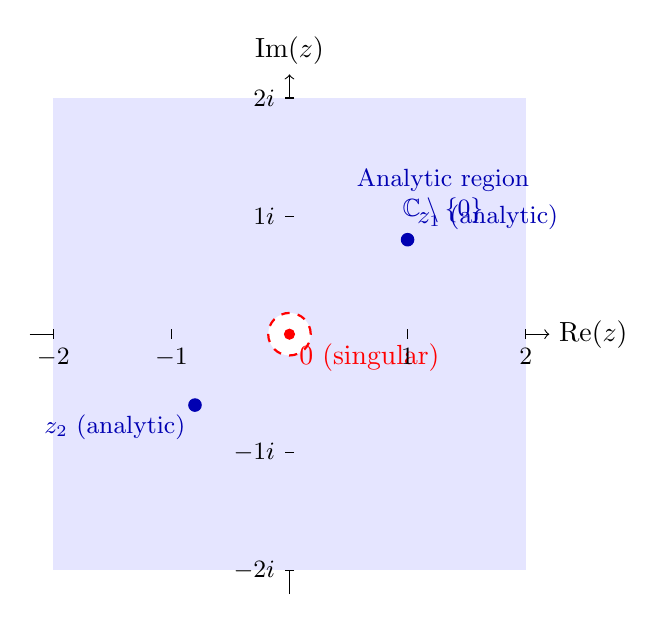
\begin{tikzpicture}[scale=1.5]
  % Axes
  \draw[->] (-2.2,0) -- (2.2,0) node[right] {$\operatorname{Re}(z)$};
  \draw[->] (0,-2.2) -- (0,2.2) node[above] {$\operatorname{Im}(z)$};

  % Shade the analytic region (full plane minus origin) with light blue
  \fill[blue!10] (-2,-2) rectangle (2,2);
  % White out a small disk around the origin to indicate non-analyticity
  \fill[white] (0,0) circle (0.18);
  \draw[red, thick, dashed] (0,0) circle (0.18);

  % Origin marker
  \filldraw[red] (0,0) circle (1.2pt) node[below right, red] {$0$ (singular)};

  % Annotate analytic region
  \node[blue!70!black] at (1.3, 1.3) {\small Analytic region};
  \node[blue!70!black] at (1.3, 1.05) {\small $\mathbb{C}\setminus\{0\}$};

  % A sample analytic point
  \filldraw[blue!70!black] (1.0, 0.8) circle (1.5pt)
      node[above right, blue!70!black] {\small $z_1$ (analytic)};

  % Another sample point
  \filldraw[blue!70!black] (-0.8, -0.6) circle (1.5pt)
      node[below left, blue!70!black] {\small $z_2$ (analytic)};

  % Tick marks
  \foreach \x in {-2,-1,1,2} {
    \draw (\x,0.04) -- (\x,-0.04) node[below] {\small $\x$};
  }
  \foreach \y in {-2,-1,1,2} {
    \draw (0.04,\y) -- (-0.04,\y) node[left] {\small $\y i$};
  }

  \node[below right] at (0,0) {};
\end{tikzpicture}
\end{center}

\textbf{Interpretation:} The blue-shaded region is where $f(z) = 1/z$ is analytic.
The red dashed circle marks an infinitesimally small exclusion around $z=0$,
the \emph{isolated singularity}. Every circle centered at $0$ with any positive
radius still encloses the singularity, so $1/z$ can never be analytic at $0$.

A second useful picture contrasts $f(z) = z^{2}$ (analytic everywhere --- the full plane is shaded) with $f(z) = \overline{z}$ (nowhere analytic --- no region shaded):

\begin{center}
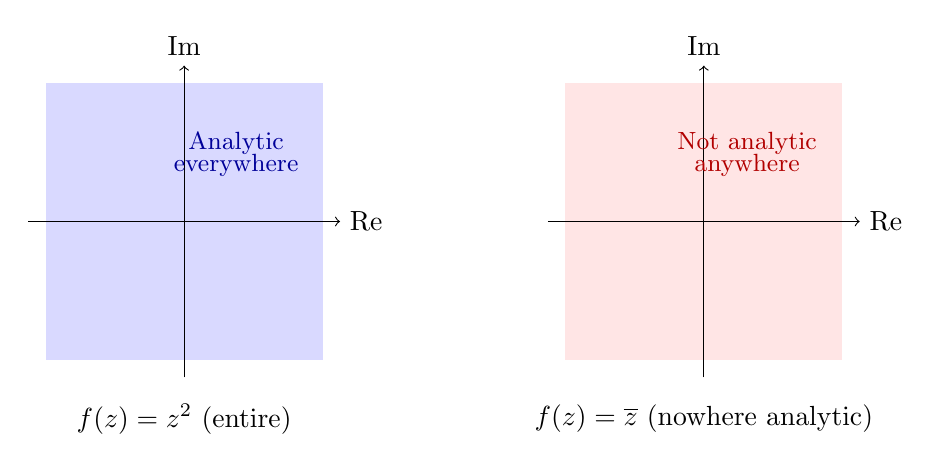
\begin{tikzpicture}[scale=1.1]
  % ---- Left: z^2 (entire) ----
  \begin{scope}[xshift=-3cm]
    \fill[blue!15] (-1.6,-1.6) rectangle (1.6,1.6);
    \draw[->] (-1.8,0) -- (1.8,0) node[right] {$\operatorname{Re}$};
    \draw[->] (0,-1.8) -- (0,1.8) node[above] {$\operatorname{Im}$};
    \node[below] at (0,-2.0) {$f(z) = z^{2}$ (entire)};
    \node[blue!60!black, font=\small] at (0.6,0.9) {Analytic};
    \node[blue!60!black, font=\small] at (0.6,0.65) {everywhere};
  \end{scope}
  % ---- Right: conj(z) (nowhere analytic) ----
  \begin{scope}[xshift=3cm]
    \fill[red!10] (-1.6,-1.6) rectangle (1.6,1.6);
    \draw[->] (-1.8,0) -- (1.8,0) node[right] {$\operatorname{Re}$};
    \draw[->] (0,-1.8) -- (0,1.8) node[above] {$\operatorname{Im}$};
    \node[below] at (0,-2.0) {$f(z) = \overline{z}$ (nowhere analytic)};
    \node[red!70!black, font=\small] at (0.5,0.9) {Not analytic};
    \node[red!70!black, font=\small] at (0.5,0.65) {anywhere};
  \end{scope}
\end{tikzpicture}
\end{center}

\begin{learnbox}{Key Takeaway}
Visual region diagrams make the notion of ``domain of analyticity'' concrete. Entire functions cover the full plane; functions with poles have punctured planes; conjugate and modulus functions have empty analytic regions.
\end{learnbox}

% ============================================================
\section{Excel Example (MANDATORY)}
% ============================================================

\textbf{Goal:} Use a spreadsheet to numerically test the C-R equations for
$f(z) = z^{2}$, i.e., $u = x^{2}-y^{2}$, $v = 2xy$, at several sampled points.

\textbf{Setup} (use a small step $h = 0.001$ for numerical partial derivatives):
\[
  u_x \approx \frac{u(x+h,y)-u(x-h,y)}{2h}, \quad
  v_y \approx \frac{v(x,y+h)-v(x,y-h)}{2h},
\]
\[
  u_y \approx \frac{u(x,y+h)-u(x,y-h)}{2h}, \quad
  v_x \approx \frac{v(x+h,y)-v(x-h,y)}{2h}.
\]

\textbf{Spreadsheet layout (columns A--K):}

\begin{center}
\begin{tabular}{cll}
\toprule
\textbf{Column} & \textbf{Header} & \textbf{Formula / Description} \\
\midrule
A & $x$ & Input value (e.g.\ 1, 2, 3) \\
B & $y$ & Input value (e.g.\ 1, 2, 3) \\
C & $u(x,y)$ & \texttt{=A2\^{}2-B2\^{}2} \\
D & $v(x,y)$ & \texttt{=2*A2*B2} \\
E & $u_x$ (numerical) & \texttt{=(((A2+0.001)\^{}2-B2\^{}2)-((A2-0.001)\^{}2-B2\^{}2))/(2*0.001)} \\
F & $v_y$ (numerical) & \texttt{=(2*A2*(B2+0.001)-2*A2*(B2-0.001))/(2*0.001)} \\
G & $u_x = v_y$? & \texttt{=IF(ABS(E2-F2)<0.0001,"YES","NO")} \\
H & $u_y$ (numerical) & \texttt{=((A2\^{}2-(B2+0.001)\^{}2)-(A2\^{}2-(B2-0.001)\^{}2))/(2*0.001)} \\
I & $-v_x$ (numerical) & \texttt{=-(2*(A2+0.001)*B2-2*(A2-0.001)*B2)/(2*0.001)} \\
J & $u_y = -v_x$? & \texttt{=IF(ABS(H2-I2)<0.0001,"YES","NO")} \\
K & Analytic? & \texttt{=IF(AND(G2="YES",J2="YES"),"YES","NO")} \\
\bottomrule
\end{tabular}
\end{center}

\textbf{Sample data rows:}

\begin{center}
\begin{tabular}{ccccccccccc}
\toprule
$x$ & $y$ & $u$ & $v$ & $u_x$ & $v_y$ & $u_x{=}v_y$? & $u_y$ & $-v_x$ & $u_y{=}{-}v_x$? & Analytic? \\
\midrule
1 & 1 & 0 & 2 & 2.000 & 2.000 & YES & $-2.000$ & $-2.000$ & YES & YES \\
2 & 3 & $-5$ & 12 & 4.000 & 4.000 & YES & $-6.000$ & $-6.000$ & YES & YES \\
0 & 0 & 0 & 0 & 0.000 & 0.000 & YES & 0.000 & 0.000 & YES & YES \\
\bottomrule
\end{tabular}
\end{center}

All rows report YES, confirming that $f(z) = z^{2}$ satisfies C-R at every sampled point.

\begin{learnbox}{Excel Takeaway}
Numerical verification of C-R equations in a spreadsheet is a quick sanity check---especially valuable for complicated functions where symbolic computation is tedious.
\end{learnbox}

% ============================================================
\section{Python Example (MANDATORY)}
% ============================================================

The following script uses \texttt{sympy} to check the Cauchy--Riemann equations
symbolically for several candidate functions and reports the domain of analyticity.

\begin{lstlisting}[language=Python, caption={Analyticity test using SymPy}]
import sympy as sp

x, y = sp.symbols('x y', real=True)

def check_CR(u_expr, v_expr, label):
    """Check Cauchy-Riemann equations for f = u + iv."""
    ux = sp.diff(u_expr, x)
    uy = sp.diff(u_expr, y)
    vx = sp.diff(v_expr, x)
    vy = sp.diff(v_expr, y)

    cr1 = sp.simplify(ux - vy)   # should be 0
    cr2 = sp.simplify(uy + vx)   # should be 0

    analytic = (cr1 == 0 and cr2 == 0)
    print(f"--- {label} ---")
    print(f"  u_x - v_y = {cr1}  (need 0)")
    print(f"  u_y + v_x = {cr2}  (need 0)")
    print(f"  Analytic (symbolic): {analytic}")
    print()

# f(z) = z^2  =>  u = x^2 - y^2,  v = 2xy
check_CR(x**2 - y**2, 2*x*y, "f(z) = z^2")
# Expected: Analytic (symbolic): True

# f(z) = conj(z)  =>  u = x,  v = -y
check_CR(x, -y, "f(z) = conj(z)")
# Expected: Analytic (symbolic): False

# f(z) = e^z  =>  u = e^x cos(y),  v = e^x sin(y)
u_ez = sp.exp(x) * sp.cos(y)
v_ez = sp.exp(x) * sp.sin(y)
check_CR(u_ez, v_ez, "f(z) = e^z")
# Expected: Analytic (symbolic): True

# f(z) = |z|^2  =>  u = x^2 + y^2,  v = 0
check_CR(x**2 + y**2, sp.Integer(0), "f(z) = |z|^2")
# Expected: Analytic (symbolic): False
# (cr1 = 2x - 0 != 0 in general)

# f(z) = 1/z (away from 0) =>  u = x/(x^2+y^2), v = -y/(x^2+y^2)
denom = x**2 + y**2
u_inv = x / denom
v_inv = -y / denom
check_CR(u_inv, v_inv, "f(z) = 1/z  (away from z=0)")
# Expected: Analytic (symbolic): True

# f(z) = sin(z) => u = sin(x)cosh(y), v = cos(x)sinh(y)
u_sin = sp.sin(x)*sp.cosh(y)
v_sin = sp.cos(x)*sp.sinh(y)
check_CR(u_sin, v_sin, "f(z) = sin(z)")
# Expected: Analytic (symbolic): True
\end{lstlisting}

\textbf{Expected output:}
\begin{verbatim}
--- f(z) = z^2 ---
  u_x - v_y = 0  (need 0)
  u_y + v_x = 0  (need 0)
  Analytic (symbolic): True

--- f(z) = conj(z) ---
  u_x - v_y = 2  (need 0)
  u_y + v_x = 0  (need 0)
  Analytic (symbolic): False

--- f(z) = e^z ---
  u_x - v_y = 0  (need 0)
  u_y + v_x = 0  (need 0)
  Analytic (symbolic): True

--- f(z) = |z|^2 ---
  u_x - v_y = 2*x  (need 0)
  u_y + v_x = 2*y  (need 0)
  Analytic (symbolic): False

--- f(z) = 1/z  (away from z=0) ---
  u_x - v_y = 0  (need 0)
  u_y + v_x = 0  (need 0)
  Analytic (symbolic): True

--- f(z) = sin(z) ---
  u_x - v_y = 0  (need 0)
  u_y + v_x = 0  (need 0)
  Analytic (symbolic): True
\end{verbatim}

\begin{learnbox}{Python Takeaway}
SymPy's symbolic differentiation makes C-R verification immediate and error-free. The script confirms which standard functions are entire and which fail analyticity, matching our hand calculations exactly.
\end{learnbox}

% ============================================================
\section{Viva Questions}
% ============================================================

\begin{enumerate}
  \item What is the difference between a function being differentiable at a
        point and being analytic at that point? Give an example that illustrates
        the distinction.

  \item Define an \emph{entire function}. Give three examples of entire functions
        and explain why each is entire.

  \item State the Cauchy--Riemann equations. Why are they necessary but not
        always sufficient for analyticity?

  \item Is $f(z) = |z|^{2}$ analytic anywhere? Prove your answer using the
        C-R equations.

  \item What is a singular point of a complex function? Distinguish between an
        isolated and a non-isolated singularity with examples.

  \item Show that $f(z) = e^{z}$ is entire by verifying the C-R equations and
        computing $f'(z)$.

  \item Can the real part of an analytic function be an arbitrary function of
        $x$ and $y$? What constraint does analyticity impose on $u(x,y)$?

  \item If $f(z)$ and $g(z)$ are analytic in a region $D$, under what condition
        is $f(z)/g(z)$ also analytic in $D$?
\end{enumerate}

% ============================================================
\section{Descriptive Questions}
% ============================================================

\begin{enumerate}
  \item State and prove the necessary conditions for a complex function
        $f(z) = u + iv$ to be analytic in a region. Illustrate with the function
        $f(z) = z^{3}$.

  \item Discuss the concept of an entire function. Show that polynomials,
        $e^{z}$, $\sin z$, and $\cos z$ are all entire functions.

  \item Explain the relationship between the Cauchy--Riemann equations and
        analyticity. Why does satisfying C-R at a single point not guarantee
        analyticity at that point? Use $f(z) = |z|^{2}$ as a counter-example.

  \item Define singular points of a complex function. Classify the singular
        points of (a) $f(z) = 1/z$, (b) $f(z) = 1/(z^{2}+4)$, and
        (c) $f(z) = e^{1/z}$.

  \item State the closure properties of analytic functions. Use these properties
        to determine the domain of analyticity of
        $f(z) = \dfrac{e^{z}\sin z}{z^{2}-1}$.
\end{enumerate}

% ============================================================
\section{Practice Problems}
% ============================================================

\begin{enumerate}
  \item Show that $f(z) = z^{4}$ is entire and find $f'(z)$.
        \textit{(Hint: Use C-R with $u = x^4 - 6x^2y^2 + y^4$, $v = 4x^3y - 4xy^3$.)}

  \item Test whether $f(z) = x^{2} + iy^{2}$ is analytic. Find the points (if
        any) where it is differentiable.
        \textit{(Hint: C-R gives $2x = 2y$, so differentiable only on the line $x = y$.)}

  \item Determine where $f(z) = \dfrac{z+1}{z^{2}+z+1}$ is analytic.
        \textit{(Hint: Find the roots of $z^{2}+z+1 = 0$ using the quadratic formula.)}

  \item Show that $f(z) = \cos z$ is entire by verifying the C-R equations for
        $u = \cos x\cosh y$, $v = -\sin x\sinh y$.
        \textit{(Hint: Differentiate each component and check $u_x = v_y$, $u_y = -v_x$.)}

  \item Prove that $f(z) = \operatorname{Re}(z)$ is nowhere analytic.
        \textit{(Hint: $u = x$, $v = 0$; $u_x = 1 \neq v_y = 0$.)}

  \item Find all singular points of $f(z) = \dfrac{z^{2}+2z+3}{(z-1)(z+2i)(z-3i)}$
        and state the domain of analyticity.
        \textit{(Hint: Singular points are $z = 1, -2i, 3i$.)}
\end{enumerate}

% ============================================================
\section{MCQs}
% ============================================================

\begin{enumerate}

  \item A function $f(z)$ that is analytic in the entire complex plane $\mathbb{C}$ is called:
  \begin{enumerate}[(a)]
    \item a harmonic function
    \item a meromorphic function
    \item \textbf{an entire function}
    \item a singular function
  \end{enumerate}
  \textit{An entire function is one that is analytic everywhere in $\mathbb{C}$ with no singularities.}

  \item The function $f(z) = \overline{z}$ is:
  \begin{enumerate}[(a)]
    \item analytic everywhere
    \item analytic only at $z = 0$
    \item analytic in the upper half-plane
    \item \textbf{nowhere analytic}
  \end{enumerate}
  \textit{$u = x$, $v = -y$ gives $u_x = 1 \neq v_y = -1$ at every point, so C-R fails everywhere.}

  \item Which of the following is an entire function?
  \begin{enumerate}[(a)]
    \item $1/z$
    \item $\tan z$
    \item $\ln z$
    \item \textbf{$e^{z}$}
  \end{enumerate}
  \textit{$e^{z}$ has no singularities in $\mathbb{C}$ and satisfies C-R everywhere; the others have singularities.}

  \item The Cauchy--Riemann equations being satisfied at a single point $z_0$ imply that $f$ is:
  \begin{enumerate}[(a)]
    \item analytic at $z_0$
    \item analytic in a neighborhood of $z_0$
    \item \textbf{at most differentiable at $z_0$, but not necessarily analytic}
    \item harmonic at $z_0$
  \end{enumerate}
  \textit{C-R at one point is necessary but not sufficient for analyticity; satisfaction throughout a neighborhood is required.}

  \item The domain of analyticity of $f(z) = \dfrac{1}{z^{2}+4}$ is:
  \begin{enumerate}[(a)]
    \item $\mathbb{C}$
    \item $\mathbb{C}\setminus\{2\}$
    \item \textbf{$\mathbb{C}\setminus\{2i, -2i\}$}
    \item $\mathbb{C}\setminus\{4\}$
  \end{enumerate}
  \textit{$z^{2}+4 = 0 \Rightarrow z = \pm 2i$; these are the only points excluded from the domain of analyticity.}

\end{enumerate}

% ============================================================
\section{Common Mistakes}
% ============================================================

\begin{mistakebox}{Common Mistakes in Analytic Functions}
\begin{center}
\begin{tabular}{p{5cm} p{5cm} p{5cm}}
\toprule
\textbf{Mistake} & \textbf{Why It Is Wrong} & \textbf{Correct Approach} \\
\midrule
Confusing ``differentiable at a point'' with ``analytic at a point'' &
Differentiability at one point requires C-R there; analyticity requires C-R in an entire neighborhood. $|z|^{2}$ is differentiable at 0 but not analytic there. &
Always check that C-R holds throughout an open neighborhood, not just at the single point. \\
\midrule
Assuming C-R at one point is sufficient for analyticity &
Analyticity requires C-R to hold (with continuous partials) in a whole open disk. One-point satisfaction is only a necessary condition for differentiability there. &
Establish C-R in a neighborhood; verify that partial derivatives are continuous in that neighborhood. \\
\midrule
Forgetting to exclude denominator zeros when stating the domain of analyticity &
A rational function $P(z)/Q(z)$ fails to be analytic (has poles) at every zero of $Q(z)$. Missing these gives an incorrect domain. &
Solve $Q(z) = 0$ and exclude those points explicitly: domain $= \mathbb{C} \setminus \{\text{zeros of } Q\}$. \\
\midrule
Claiming $f(z) = \overline{z}$ is analytic because it maps $\mathbb{C}$ to $\mathbb{C}$ &
Analyticity is not about the codomain but about complex differentiability. $\overline{z}$ reflects the plane and reverses orientation---it fails C-R everywhere. &
Check C-R: $u_x = 1$, $v_y = -1$. Since $1 \neq -1$, $\overline{z}$ is nowhere analytic. \\
\midrule
Using $\int$ instead of $\oint$ for closed-contour integrals involving analytic functions &
$\oint$ explicitly denotes a closed contour; using $\int$ obscures the topology and can lead to incorrect application of Cauchy's theorem. &
Always write $\oint_{C} f(z)\,dz$ for integrals over closed contours. \\
\bottomrule
\end{tabular}
\end{center}
\end{mistakebox}

% ============================================================
\section{Quick Recap}
% ============================================================

\begin{learnbox}{Quick Recap --- Analytic Functions}
\begin{itemize}
  \item A function is \textbf{analytic at $z_0$} if it is complex-differentiable
        at every point of some open neighborhood of $z_0$; mere differentiability
        at $z_0$ alone is insufficient.

  \item A function analytic on all of $\mathbb{C}$ is called \textbf{entire};
        examples include $z^{n}$, $e^{z}$, $\sin z$, $\cos z$.

  \item A \textbf{singular point} $z_0$ is where analyticity fails yet every
        neighborhood of $z_0$ contains analytic points; isolated singularities
        are classified as removable, poles, or essential.

  \item The practical test: C-R equations $u_x = v_y$, $u_y = -v_x$ with
        \textbf{continuous partial derivatives throughout a neighborhood} $\Rightarrow$
        analytic in that neighborhood.

  \item Analytic functions are closed under $+$, $-$, $\times$, $\div$ (denominator
        non-zero), and composition; they are infinitely differentiable and admit
        local power-series representations.

  \item $f(z) = \overline{z}$, $|z|^{2}$, $\operatorname{Re}(z)$ fail C-R
        everywhere (or almost everywhere) and are not analytic in any region.

  \item For rational functions $P(z)/Q(z)$, the domain of analyticity is
        $\mathbb{C}$ minus the zeros of $Q(z)$.

  \item The domain of analyticity is always an \textbf{open set}; requiring an
        open neighborhood is what makes analyticity genuinely stronger than
        pointwise differentiability.
\end{itemize}
\end{learnbox}

\end{document}
